\subsection{Evaluación de los métodos}

\subsubsection{Único $b$}
Nuestro primer análisis de los métodos utilizados para la resolución del problema va a consistir en una teórica. 

La resolución mediante el método de eliminación Gaussiana tiene dos partes, la primera es la eliminación gaussiana propiamente dicha, que tiene un costo de $O(k^3)$ flops, donde $k$ es la cantidad de filas (y columnas) de la matriz y la segunda es el algoritmo llamado \emph{backwards substitution}, que tiene un costo de $O(k^2)$ flops.

La resolución mediante el método de factorización LU tiene tres partes, la primera es obtener la factorización LU de la matriz en cuestión, que tiene un costo de $O(k^3)$, y luego aplicar \emph{forward substitution} y \emph{backward substitution}, cada uno con un costo de $O(n^2)$ flops.



Para medir los tiempos de ambas implementaciones decidimos hacer dos experimentos separados, sin embargo similares. 
En uno fijamos una cantidad de radios y movemos la cantidad de angulos, y en el otro al revés.
Lo hicimos así para que las dimensiones de la matriz (ancho o alto, dado que son iguales porque es cuadrada) crezca linealmente, ya que si hacemos variar ángulos y radios al mismo tiempo, las dimensiones dejan de crecer linealmente.
Queremos que las dimensiones crezcan linealmente para que los resultados se entiendan mejor, dado que una escala lineal es, generalmente, más naturales a la vista.


\begin{figure}[H]
\centering
\begin{minipage}{0.48\textwidth}
  \centering
    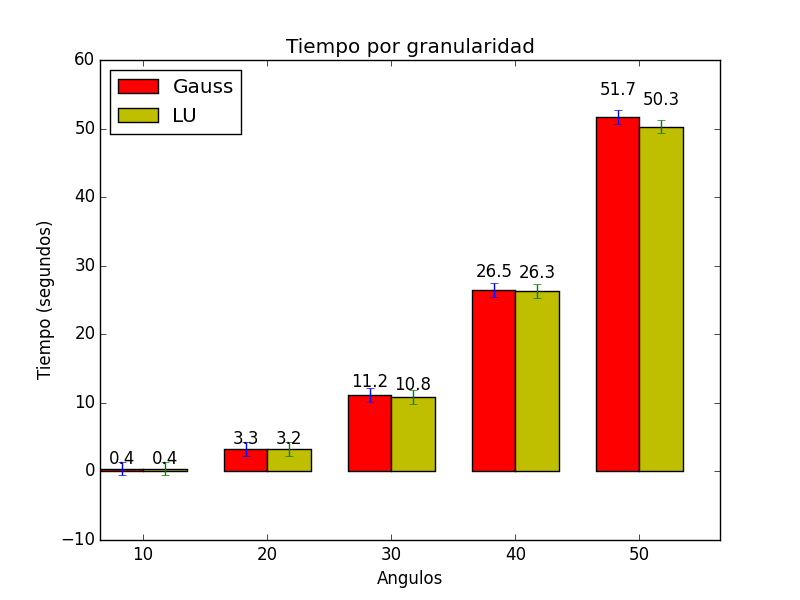
\includegraphics[width=1\textwidth]{imgs/tiempos_vanilla_angulos.png}
  \caption{\footnotesize{Tiempo tomado por la nuestra implementación de eliminación gaussiana y de factorización LU para resolver el problema. La granularidad de radios está fija en 40 y la de ángulos se indica en el eje $x$. La barra principal indica el promedio, y el segmento indica la desviación standard.}}
  \label{fig:tiempo1}
\end{minipage}%
\hspace{0.03\textwidth}
\begin{minipage}{0.48\textwidth}   
  \centering
    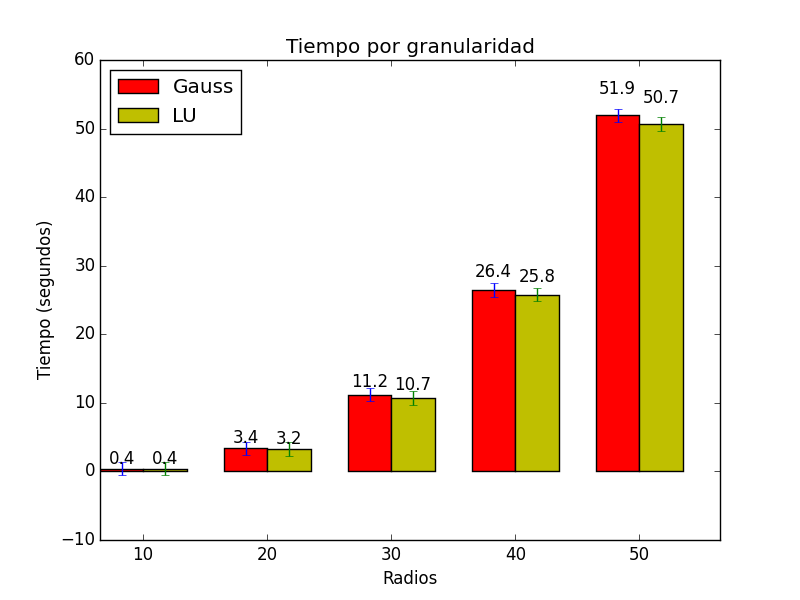
\includegraphics[width=1\textwidth]{imgs/tiempos_vanilla_radios.png} 
  \caption{\footnotesize{Tiempo tomado por la nuestra implementación de eliminación gaussiana y de factorización LU para resolver el problema. La granularidad de ángulos está fija en 40 y la de radios se indica en el eje $x$. La barra principal indica el promedio, y el segmento indica la desviación standard.}}
  \label{fig:tiempo2}
\end{minipage}
\end{figure}



Como se ve en las figuras \ref{fig:tiempo1} y \ref{fig:tiempo2}, las performances entre las implementaciones son realmente similares. También puede observarse algo que nos llamó la atención, que es que el método por eliminación gaussiana tuvo consistentemente peor performance que LU, contradiciendo parcialmente el análisis a priori. Sin embargo, la diferencia es mínima: siempre menor al 3\%.

Por esta razón no creemos que sea algo importante a tener en cuenta, y podríamos atribuirlo a optimizaciones del compilador, dado que los códigos son realmente parecidos (de hecho hicimos nuestra implementación de la factorización LU sobre nuestra implementación de eliminación gaussiana), y las partes que son diferentes le agregan complejidad a la factorización LU.

Por eso lo atribuimos a cuestiones relacionadas con la optimización en tiempo de compilación y no a errores en las mediciones, dado que los tests fueron corridos varias veces por el hecho de que estos resultados eran llamativos.


Por otro lado, vemos que dividir entre ángulos y radios no hace diferencia en la performance, dado que como esperabamos, el runtime solamente depende del tamaño de la matriz, es decir $n (m+1)$, que en ambos gráficos es igual columna a columna.


Ahora es el turno de las implementaciones que aprovechan que la matriz es banda.
La diferencia es enorme. Para comparar rápidamente, podemos usar una tabla:


\begin{figure}[H]
\centering
\begin{tabular}{|r | c  c  c  c|}
\hline
  \textbf{Implementación} & Gauss & Gauss Banda & LU & LU Banda\\ \hline
  \textbf{Tiempo (segundos)} & 26.24 & 0.98 & 25.53 & 1.04 \\
\hline
\end{tabular}

  \caption{\footnotesize{Tiempo promedio tomado por las implementaciones para resolver un sistema con $n = m+1 = 40$.}}
  \label{fig:tiempocomp}
\end{figure}

Con la Figura \ref{fig:tiempocomp} se observa como la diferencia entre las implementaciones \emph{vanilla} y las optimizadas es abismal, superando el 2600\%.

Esta tabla no pretende analizar las implementaciones optimizadas, simplemente probar la diferencia de rendimiento que se obtiene.

A continuación analizaremos las implementaciones optimizadas.

[ACA ANALIZAMOS LA COMPLEJIDAD O LO REPETIMOS CORTITO]

\begin{figure}[H]
\centering
\begin{minipage}{0.48\textwidth}
  \centering
    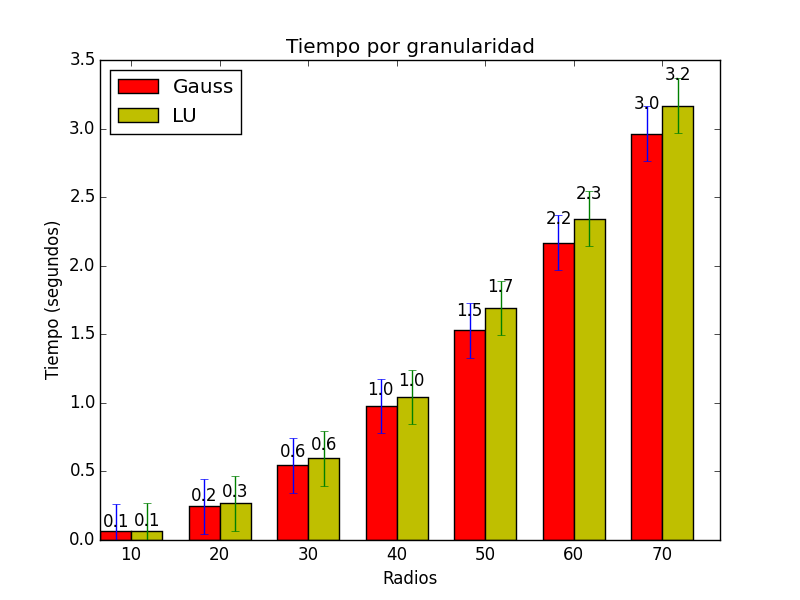
\includegraphics[width=1\textwidth]{imgs/tiempos_opt_angulos.png}
  \caption{\footnotesize{Tiempo tomado por la nuestra implementación optimizada de eliminación gaussiana y de factorización LU para resolver el problema. La granularidad de radios está fija en 40 y la de ángulos se indica en el eje $x$. La barra principal indica el promedio, y el segmento indica la desviación standard.}}
  \label{fig:tiempoopt1}
\end{minipage}%
\hspace{0.03\textwidth}
\begin{minipage}{0.48\textwidth}   
  \centering
    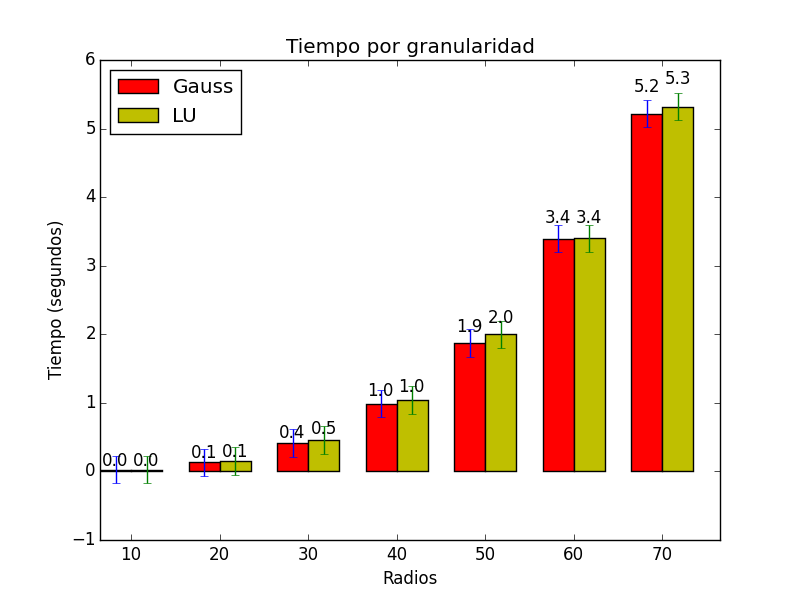
\includegraphics[width=1\textwidth]{imgs/tiempos_opt_radios.png} 
  \caption{\footnotesize{Tiempo tomado por la nuestra implementación optimizada de eliminación gaussiana y de factorización LU para resolver el problema. La granularidad de ángulos está fija en 40 y la de radios se indica en el eje $x$. La barra principal indica el promedio, y el segmento indica la desviación standard.}}
  \label{fig:tiempoopt2}
\end{minipage}
\end{figure}


Los resultados que se ven en las Figuras \ref{fig:tiempoopt1} y \ref{fig:tiempoopt2} son muy interesantes. Primero notemos que como los procesos de eliminación gaussiana y factorización LU ambos consumen menos tiempo, se nota más la ventaja que le saca gauss a LU con un solo $b$, dado que los procesos de substitución empiezan a pesar asintóticamente.


Como la complejidad de los algoritmos optimizados es $O(\text{radios}^3   \text{angulos})$, en los experimentos se refleja que es mucho más caro aumentar la granularidad con respecto a los radios que con respecto a los ángulos.

\subsubsection{Múltiples $b$'s}

Cuando buscamos simular un escenario similar al experimento anterior, pero donde las condiciones de borde (temperaturas interiores y exteriores) cambian en distintos instantes de tiempo, la situación es muy distinta. Aquí esperaríamos ver el verdadero poder de la factorización LU.

Por esta razón, esperamos que la implementación de la factorización LU supere ampliamente a la de la eliminación Gaussiana, dado que en la Gaussiana se paga un costo cúbico cada vez que se quiere resolver el sistema, mientras que en con la factorización LU el costo cúbico se paga solo una vez.

Por esta razón se puede decir que, para muchas instancias, el costo de resolver $Ax = b$ es cúbico para la eliminación gaussiana y cuadrático amortizado para la factorización LU.

\begin{figure}[H]
\centering  
 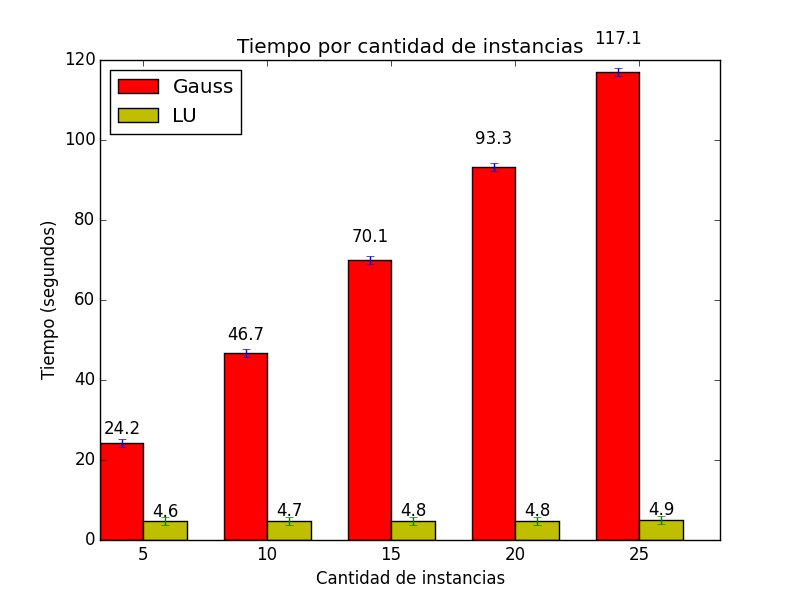
\includegraphics[width=0.6\textwidth]{imgs/tiempos_ninst.png}
 \caption{\footnotesize{Tiempo tomado por la nuestra implementación de eliminación gaussiana y de factorización LU para resolver el problema para varias instancias de $n = m+1 = 30$. La barra principal indica el promedio, y el segmento indica la desviación standard.}}
\label{fig:tiemponinst}
\end{figure}


En los resultados se refleja lo que esperabamos. Como se ve en la figura \ref{fig:tiemponinst}, luego de aplicar la factorización LU, el costo que hay que pagar para resolver cada sistema es muy poco, lo cual permite una excelente performance.

Por otra parte, se observa que el tiempo que le toma a la eliminación gaussiana resolver $n$ instancias, es también es lineal en la cantidad de instancias, pero con una pendiente mucho mayor, lo cual confirma más aún nuestras expectativas derivadas de la teoría.

En cuanto a las implementaciones optimizadas, esperamos que su comportamiento sea similar a los resultados anteriores.

\begin{figure}[H]
\centering  
 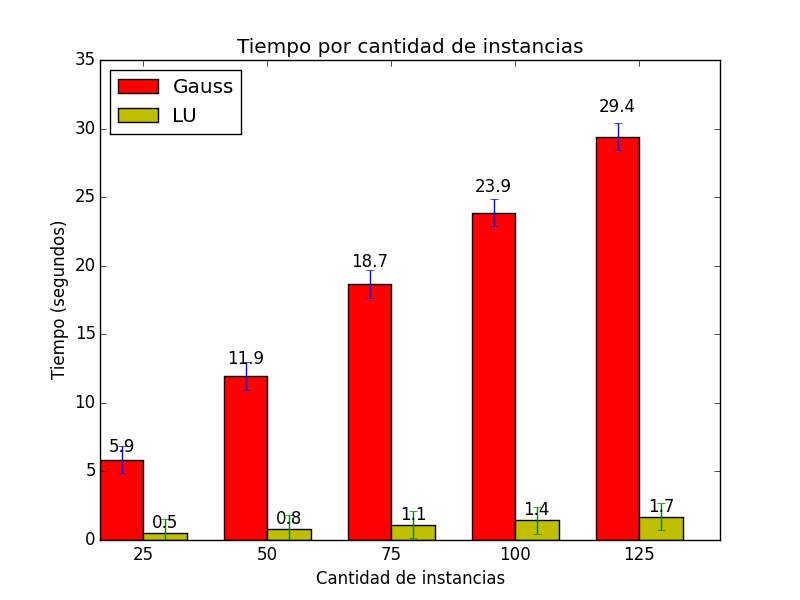
\includegraphics[width=0.6\textwidth]{imgs/tiempos_ninst_opt.png}
 \caption{\footnotesize{Tiempo tomado por la nuestra implementación optimizada de eliminación gaussiana y de factorización LU para resolver el problema para varias instancias de $n = m+1 = 30$. La barra principal indica el promedio, y el segmento indica la desviación standard.}}
\label{fig:tiemponinstopt}
\end{figure}

Como se observa en la Figura \ref{fig:tiemponinstopt}, confirmamos nuestras expectativas. Se observa, al igual que antes, que la implementación optimizada de Gauss crece linealmente con respecto a la cantidad de instancias del problema entradas, al igual que la implementación de la factorización LU, sólo que esta ultima lo hace con una pendiente mucho menor.



